\documentclass[12pt,a4paper]{article}
\title{%
  Kjemiøving 1 \\
  \large IFYKJT1001 - Fysikk/Kjemi \\
  }
\author{Gunnar Myhre, BIELEKTRO}

\usepackage[utf8]{inputenc}
\usepackage[norsk]{babel}
\usepackage{amsmath}
\usepackage{siunitx}

\usepackage{graphicx}
\graphicspath{ {./images} }

\setlength\parindent{0pt}

\begin{document}
  \maketitle

  \section*{Oppgåve 1}
    \subsection*{a)}
    I første omgong kan vi tenke på atomet som ein kjerne av protoner
    $\textbf{P}^+$ og nøytroner \textbf{N} med elektroner $\textbf{e}^-$ i bane
    rundt kjerna. Elektronene går i bane i forskjellige energinivåer, eller \textit{skal},
    og spesielt mengden elektroner i ytterste skal (\textit{valenselektroner}) bestemmer
    dei kjemiske eigenskapane til atomet.
    \begin{figure}[!h]
      \begin{center}
        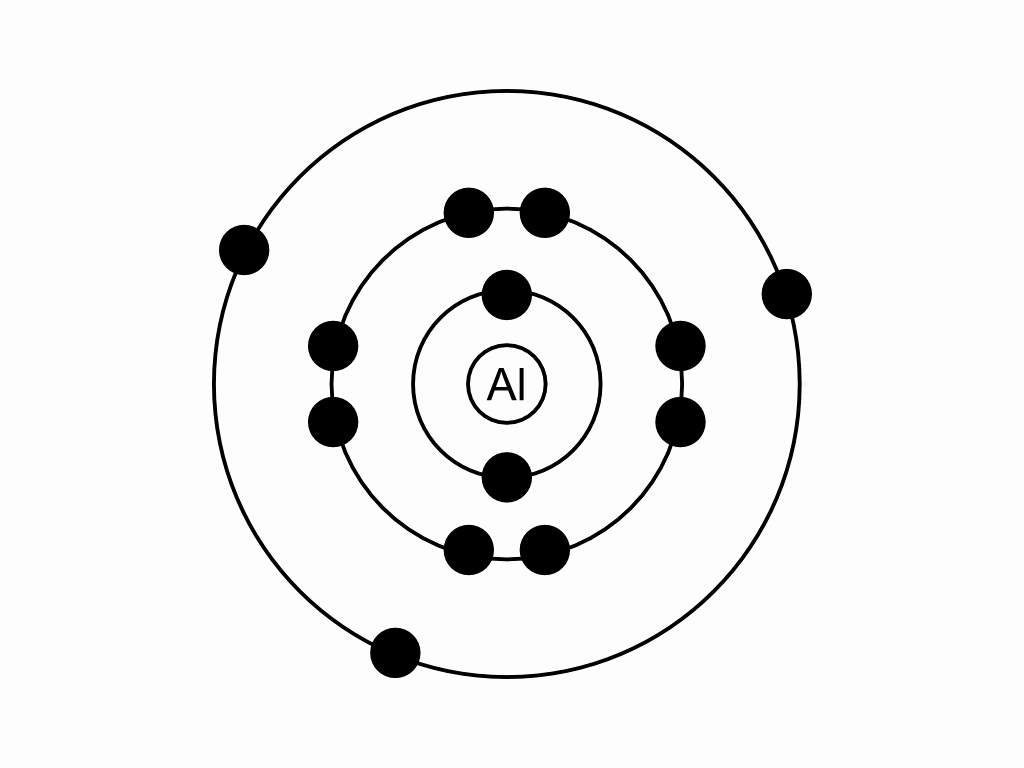
\includegraphics[scale=.1]{kj_01_bohr_al}
        \caption{Bohr-modell eller skalmodell av eit atom, her \textit{aluminium}.}
      \end{center}
    \end{figure}

    Ein modell som passer betre opp mot eksperimentelle data er orbitalmodellen. Her 
    går ikkje elektronene i bane rundt kjerna, men vi beskriver derimot ei
    \textit{elektronsky}, som er ein sannsynlighetsfunksjon av kor vi kan finne
    elektronene til einkvar tid. Orbitalene har tridimensjonal, ballongaktig utstrekning
    og er symmetriske om dei kartesiske aksene. Dei første orbitala har navn $1s$, $2s$,
    $2p$ og $3s$.
    
    \begin{figure}[!htb]
      \begin{center}
        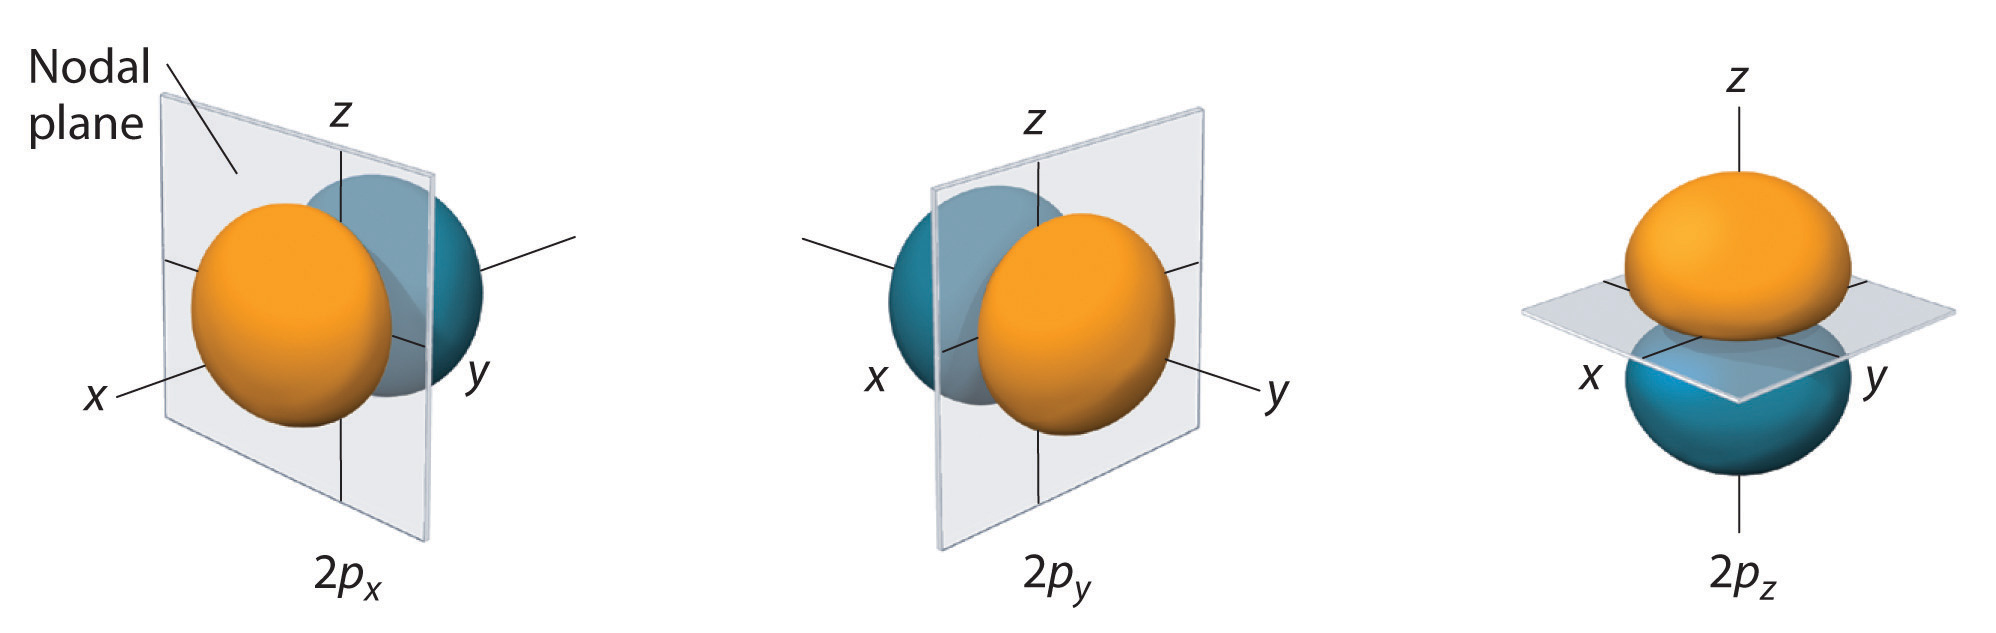
\includegraphics[scale=.08]{kj_01_orbital}
        \caption{2p-orbitalet, som ofte inneholder elektron 5 til 10}
      \end{center}
    \end{figure}

    \newpage


    \subsection*{b)}
    Natrium har atomnummer 11 og har derfor 11 protoner i kjerna. I uionisert form vil eit
    natriumatom også ha 11 elektroner.
    \begin{figure}[!h]
      \begin{center}
        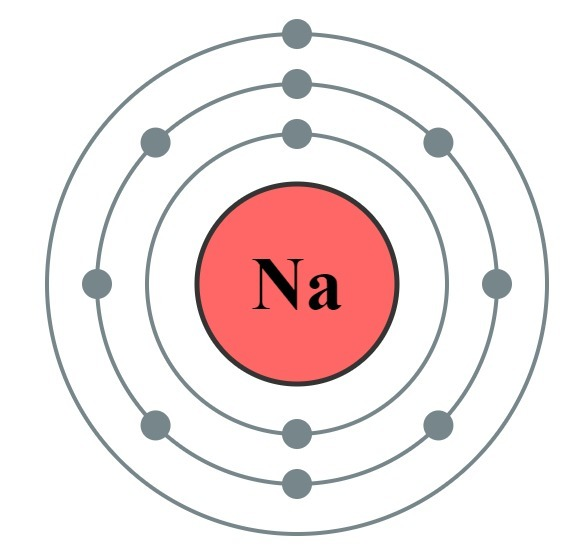
\includegraphics[scale=.08]{kj_01_bohr_na}
        \caption{Natriumatom.}
      \end{center}
    \end{figure}

  \section*{Oppgåve 2}
    \subsection*{a)}
    $^{235}_{92}U$ har 235 nukleoner og 92 protoner, det er derfor snakk om uran.
    \begin{equation}
      235 - 92 P^+ = 143 N
    \end{equation}


    \subsection*{b)}
    Karbon-14 kan vi skrive $^{14}_6 C$. Denne isotopen har $14-6= 8$ nøytroner i kjerna.


    \subsection*{c)}
    Dei tri isotopane av hydrogen er
    \begin{itemize}
      \item Protium $^1_1 H \rightarrow 0 N$
      \item Deuterium $^2_1 H \rightarrow 1N$
      \item Tritium $^3_1 H \rightarrow 2N$
    \end{itemize}
    Alle desse isotopane er fortsatt hydrogen, sidan dei har \textit{eitt} proton i kjerna.


  \section*{Oppgåve 3}
    \begin{center}
      \begin{tabular}{|c|c|c|c|}
        \hline
        Isotop & Atomnummer & Protoner & Nøytroner  \\
        \hline
        $^{23}Na$ & $11$ & $11$ & $12$ \\
        \hline
        $^{26}Mg$ & $12$ & $12$ & $14$ \\
        \hline
        $^{127}I$ & $53$ & $53$ & $74$ \\
        \hline
      \end{tabular}
    \end{center}


  \section*{Oppgåve 4}
    Periodesystemet er bygd opp slik at gruppene ($\downarrow$) viser antal valenselektroner
    (elektroner i ytterste elektronskal) og periodane ($\rightarrow$) viser antal energinivå
    (orbitalgrupper/elektronskal).
    \begin{itemize}
      \item Alkalimetall: Gruppe 1, ett valenselektron
      \item Jordalkalimetall: to valenselektron
      \item Halogener: sju valenselektron
      \item Edelgassar: åtte valenselektron (ytterste elektronskal er fyllt)
      \item Innskotsmetall er lausare definert som den store gruppa metaller i midten.
    \end{itemize}


  \section*{Oppgåve 5}
    $Li^+$, $F^-$, $K^+$, $Na^+$, $Br^-$, $Mg^{2+}$, $Ca^{2+}$, $O^{2-}$ og $Cl^+$

  \section*{Oppgåve 6}
    \begin{center}
      \begin{tabular}{|c|c|c|c|c|}
        \hline
        Atomnummer & Protoner & Elektroner & Ioneladning & Symbol \\
        \hline
        $16$  &  $16$  &  $18$  &  $2-$  &  $S^{2-}$ \\
        \hline
        $12$  &  $12$  &  $10$  &  $2+$  &  $Mg^{2+}$ \\
        \hline
        $13$  &  $13$  &  $10$  &  $3+$  &  $Al^{3+}$ \\
        \hline
        $35$  &  $35$  &  $36$  &  $1-$  &  $Br^{+}$ \\
        \hline
      \end{tabular}
    \end{center}


  \section*{Oppgåve 7}
    \subsection*{a)}
    I ein kovalent binding mellom to atomer er valenselektronene delt mellom
    atoma for å fylle opp ytterste elektronskal. Forskjelen i
    elektronegativitet mellom dei to atoma bestemmer om bindinga er polar eller
    upolar.
    \begin{itemize}
      \item $0 < \Delta EN < 0,4 \rightarrow$ upolar, kovalent binding
      \item $0,4 < \Delta EN < 2,0 \rightarrow$ polar, kovalent binding
      \item $2,0 < \Delta EN \rightarrow$ ionebinding
    \end{itemize}

    \subsection*{b)}
    I ein ionebinding er forskjelen i elektronegativitet såpass stor at
    elektroner vert permanent overført. For eksempel vil i $NaCl$ vil $Cl$
    trekke såpass mykje meir på valenselektronet til $Na$ at det går inn i
    kloratomets orbital, og dermed danner eit anion og kation $Cl^-$ og $Na^+$.

    \subsection*{c)}
    Forbindelsen mellom klor (ikkje-metall) og sink (metall) vil vi anta er ein ionebinding.
    Klor har sju valenselektroner og sink har to valenselektroner, så det er rimelig å
    anta at den kjemiske forbindelsen vi er ute etter er $ZnCl_2$


  \section*{Oppgåve 8}
    I metallbindinger er alle elektronene delokaliserte, og beveger seg fritt rundt i metallet.
    Vi snakker ofte om ein \textit{sjø} av valenselektroner som beveger seg mellom
    alle ionekjernene, i motsetning til eit enkelt metallatom der elektronene vil ligge i
    orbitaler rundt atomkjerna.
    \bigskip

    Dette gjev oss dei karakteristiske eigenskapane til metaller, som høg elektrisk og
    termisk konduktivitet.

  \newpage


  \section*{Oppgåve 9}
    Finner verdiar for elektronegativitet og anslår bindingstype
    \begin{itemize}
      \item $NaBr: \Delta EN = 2,8-0,9=1,9 \rightarrow polar kovalent$
      \item $CO: \Delta EN = 3,5-2,5=1,0 \rightarrow polar kovalent$
      \item $CsCl: \Delta EN = 3,0-0,7=2,3\rightarrow ionebinding$
    \end{itemize}


  \section*{Oppgåve 10}
    \begin{itemize}
      \item Brom, $Br_2$
      \item Hydrogenbromid, $HBr$
      \item Karbonmonoksid, $CO$
      \item Karbondioksid, $CO_2$
      \item Ammonium, $NH_4^+$
    \end{itemize}

\end{document}
